\chapter{Introduction}
\section{Multipath in Aeronautical Telemetry}
Multipath interference is one of the dominant causes for link loss in aeronautical telemetry.
Strong multipath interference occurs in aeronautical telemetry when the transmitted signal is received from multiple paths because a test article is in a low elevation angle scenario as shown in Figure \ref{fig:multipath}.
Receivers use equalizers to combat multipath but often the transmitted information can not be recovered.
Equalizers have been studied to combat multipath interference in aeronautical telemetry \cite{rice-afran-saquib:2014,rice-afran-saquib-cole-rhodes-moazzami:2014}.

There are two types of equalizers, blind and data-aided.
Blind equalizers combat multipath using known properties of the transmitted signal but no knowledge of the data or multipath channel.
Data-aided equalizers require knowing something about the received signal.
One method of providing data that can be used in data-aided equalization is for the transmitter to periodically insert a known bit sequence called a ``pilot'' into the data stream.
The receiver compares the received signal with a locally stored copy to estimate parameters such as multipath channels, frequency offsets, phase offsets and noise variance.
Data-aided equalizers are finite impulse response filters (FIR). The impulse response of the FIR filters are computed based on the estimated parameters to better mitigate multipath.
\begin{figure}
	\centering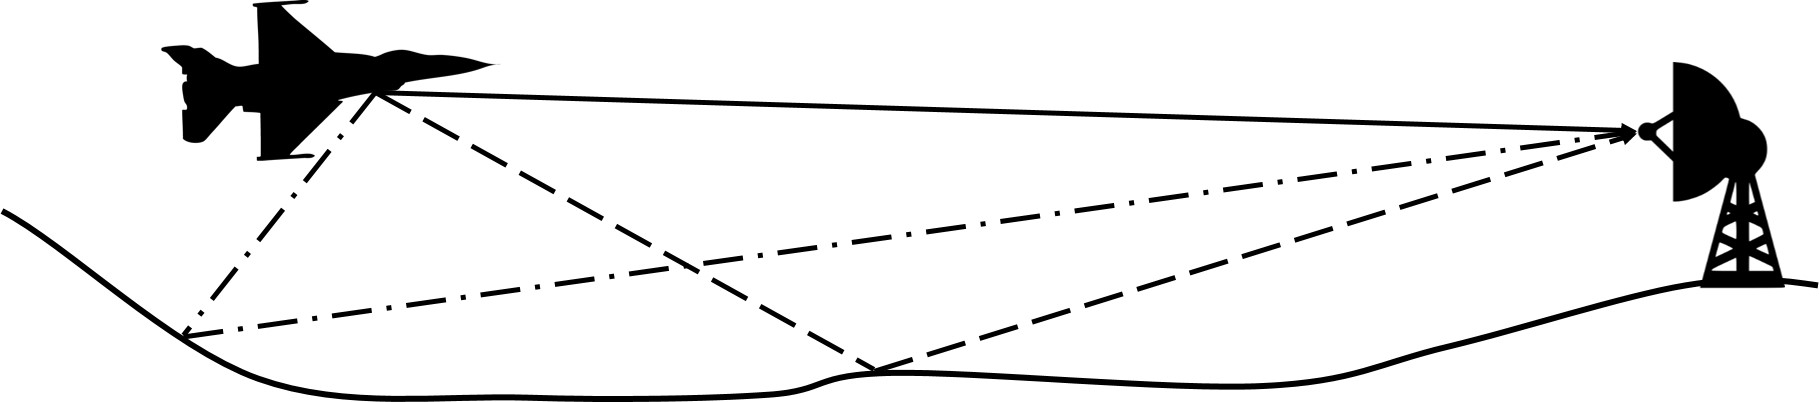
\includegraphics[width=12.11in/100*50]{figures/intro/Picture1.jpg}
	\caption{Multipath can occur when a signal is received multiple paths like line-of-sight or ground bounce or reflections.}
	\label{fig:multipath}
\end{figure}

\clearpage
\section{Preamble Assisted Equalization Project}
Data-aided equalization in aeronautical telemetry has been studied and tested by the Preamble Assisted Equalization (PAQ) project \cite{paq-phase1-report:2014}.
The PAQ project built a TRL 6 system that compares five data-aided equalizers to blind equalization and no equalization \cite{frerkingjpl}.
Bit error statistics were be used as the figure or merit for the equalization algorithms.
Live flight tests were conducted at Edwards AFB in March and June 2016.
The five data-aided equalizers the PAQ project studied are
\begin{itemize}
\item zero-forcing (ZF) equalizer
\item minimum mean square Error (MMSE) equalizer
\item MMSE initialized constant modulus algorithm (CMA) equalizer
\item frequency domain equalizer one (FDE1)
\item frequency domain equalizer Two (FDE2).
\end{itemize}
\subsubsection{Hardware}
\label{sec:hardware}
A block diagram of the PAQ project physical system is shown in Figure \ref{fig:hardwareblock}.
\begin{figure}
	\centering\includegraphics[width=11.58in/100*55]{figures/systemOverview/hardwareblock.pdf}
	\caption{A block diagram of the physical PAQ project hardware. The components inside the rack mounted server are in the dashed box. All the components in the dashed and dotted box are housed in a rack mounted case.}
	\label{fig:hardwareblock}
\end{figure}
A picture of the physical components is shown in Figure \ref{fig:HostSystem}.
\begin{figure}
	\centering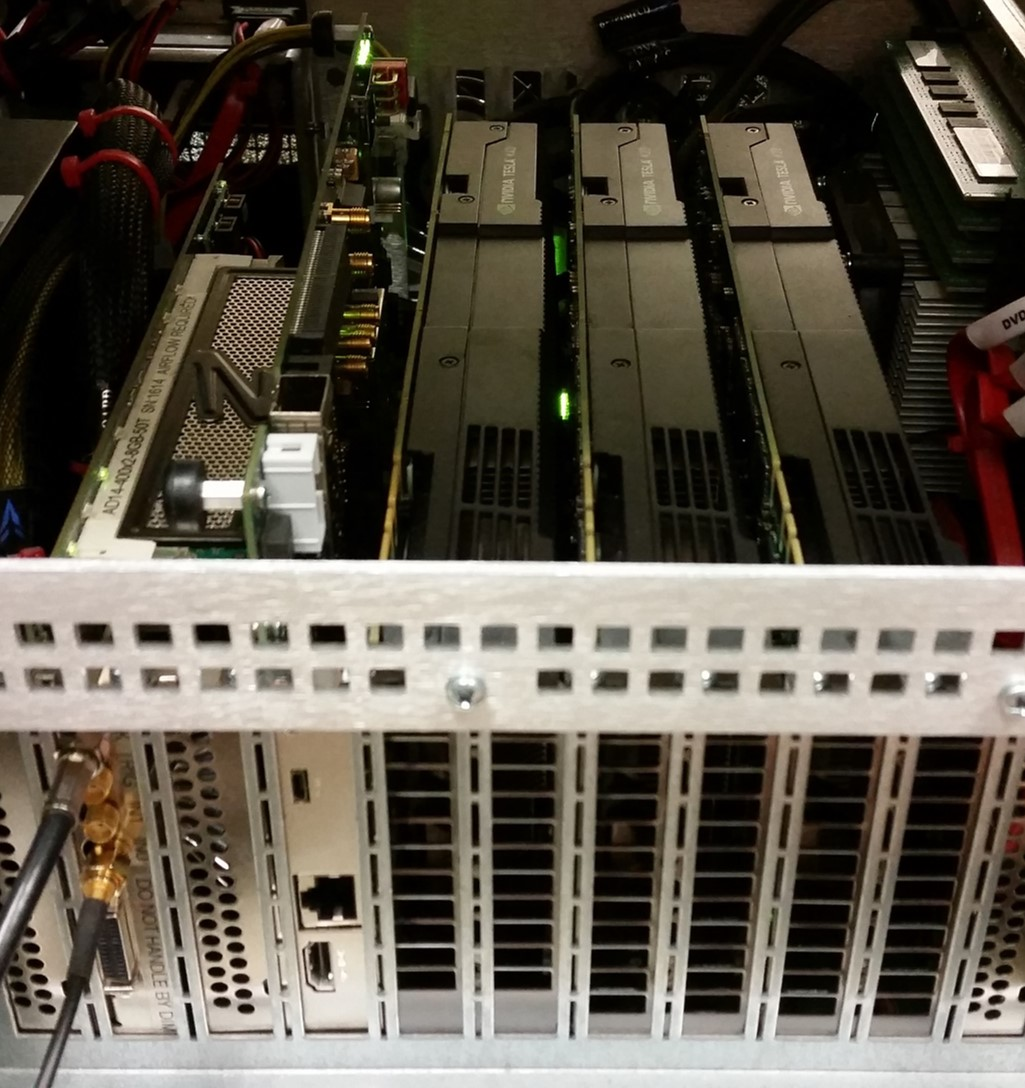
\includegraphics[scale=0.55]{figures/systemOverview/HostSystem.jpg}
	\caption{A picture of the physical PAQ project hardware. Right: Components in the dashed and dotted box from Figure \ref{fig:hardwareblock}. Left: Components in dashed box in Figure \ref{fig:hardwareblock}. Note that the T/M Receiver is not pictured.}
	\label{fig:HostSystem}
\end{figure}
The major components, and their functions are summarized in the following.
\begin{itemize}
	\item The \textbf{T/M mixer} down-converts from L or C band RF to IF (70 MHz) then applies an anti-aliasing filter.
	%
	\item The \textbf{rack mounted server} is a high powered computer that houses an ADC, a FPGA and three GPUs 		slotted into a 32 pin PCIe bus.
	\item The \textbf{ADC} produces 14-bit samples of the real-valued bandpass signal
	centered at IF sampled at $93\nicefrac{1}{3}$ Msamples/s.
	The samples are transferred to the host CPU via the PCIe bus.
	%
	\item The \textbf{host CPU} initiates memory transfers between itself and the ADC, GPUs and FPGA via the PCIe 	bus. 
	The host CPU also launches the digital signal processing algorithms on the GPUs.
	%
	\item The three \textbf{GPUs} are where all the detection, estimation, equalization and demodulation resides.
While the CPU has one to eight powerful processors, GPUs have thousands of small less powerful processors that work in parallel. The signal processing is done in GPUs rather than FPGAs or a CPU because programming GPUs is faster and easier than programming FPGAs and CPUs do not prosess the required processing power.
	%
	\item The \textbf{FPGA} receives all the bit streams from the host CPU via the PCIe bus then clocks each 			stream out in parallel to the BERT for BER testing.
	%
	\item The bit error rate tester (\textbf{BERT}) counts the errors in each input bit stream by comparing the 		streams to a PN sequence.
	%
	\item The \textbf{T/M Receiver} outputs bit streams for blind equalization and no equalization for 					BER comparison.
\end{itemize}
%A picture of the rack mounted physical system is shown in Figure \ref{fig:rack}.
%\begin{figure}
%	\centering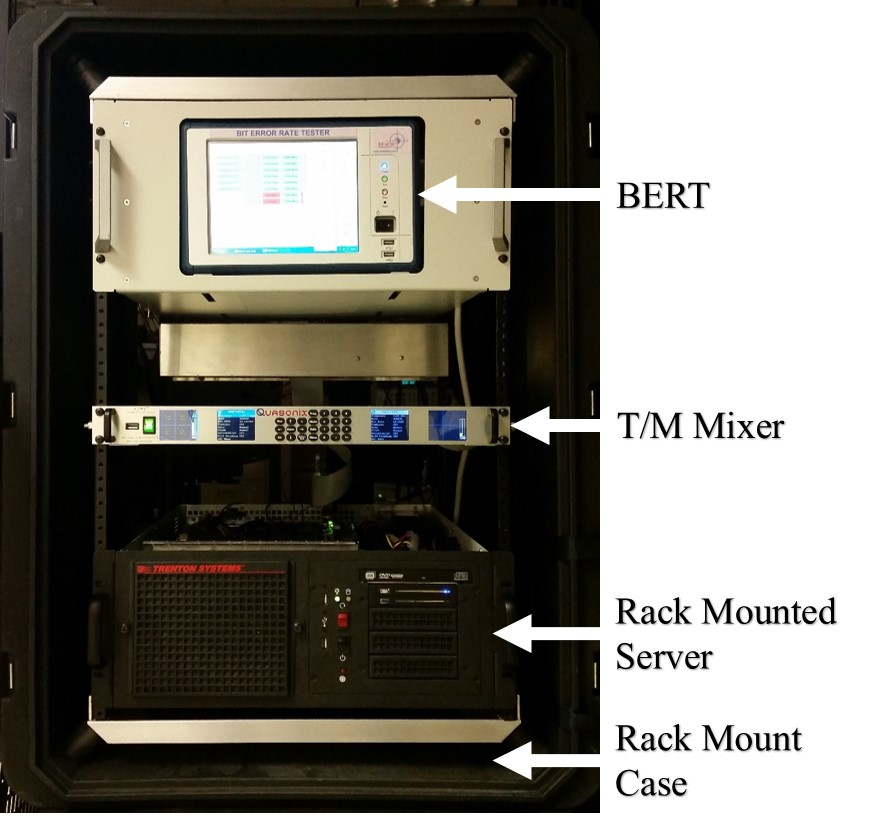
\includegraphics[scale=0.55]{figures/systemOverview/rack.jpg}
%	\caption{A picture of the physical PAQ project hardware. Note that the T/M Receiver is not pictured.}
%	\label{fig:rack}
%\end{figure}
%A picture of the components inside the rack mounted server is shown in Figure \ref{fig:rack}.
%\begin{figure}
%	\centering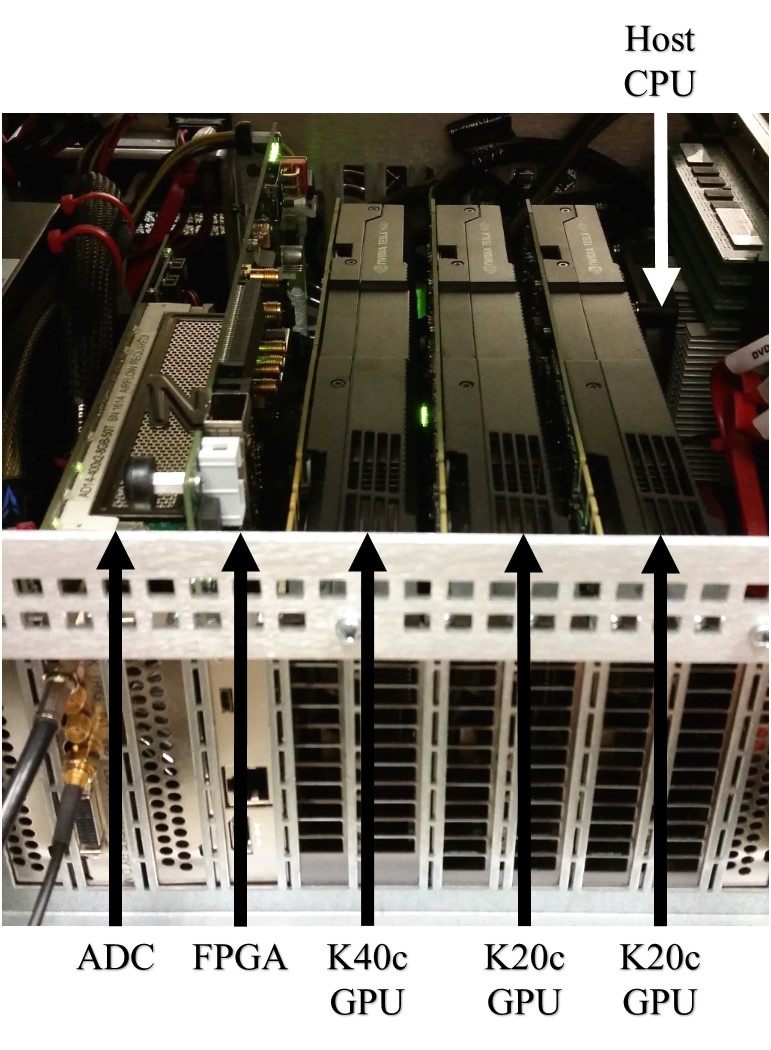
\includegraphics[scale=0.55]{figures/systemOverview/server.jpg}
%	\caption{A pictureof the components inside the rack mounted server.}
%	\label{fig:server}
%\end{figure}

To enable data-aided equalization, the PAQ project bit stream has a packetized structure shown in Figure \ref{fig:packetStructure_intro}.
The bit stream has a pilot bit sequence, in the form of the iNET preamble and ASM, periodically inserted into the data bits.
\begin{figure}
	\centering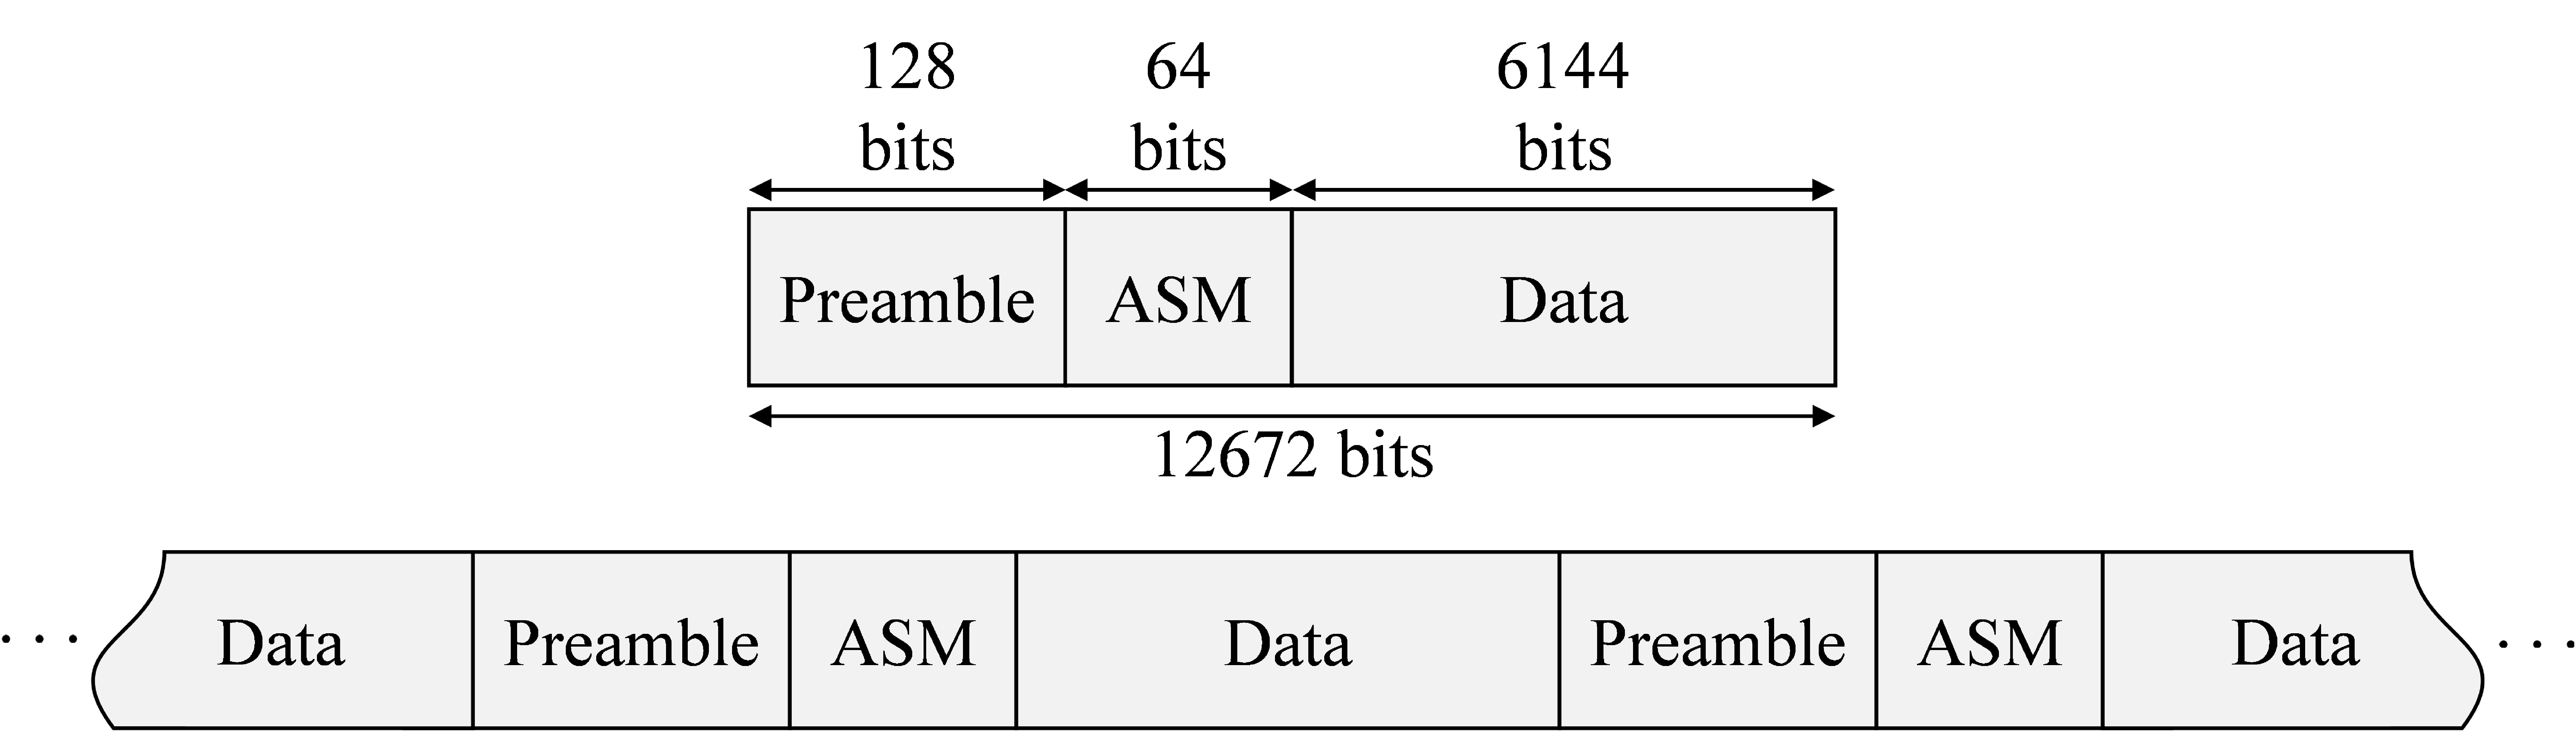
\includegraphics[width=9.47in/100*55]{figures/intro/packetSturcture.pdf}
	\caption{A diagram showing the PAQ packetized sample structure.}
	\label{fig:packetStructure_intro}
\end{figure}
The iNET preamble comprises eight repetitions of the 16-bit sequence $\text{CD98}_\text{hex}$ and the ASM field is
\begin{equation}
\text{034776C7272895B0}_\text{hex}.
\end{equation}
The data payload is a known length-$(2^{11} - 1)$ PN sequence.
Each packet contains $128$ preamble bits, $64$ ASM bits and $6{,}144$ data bits making each iNET packet $6{,}336$ bits.
The data bits modulate a SOQPSK-TG carrier at $10$ Mbits/second.
With the preamble and ASM periodically inserted, the over the air bit rate is $10.3125$ Mbits/second.

After modulation, the transmitted signal experiences multipath interference modeled as the channel $h(t)$.
The transmitted signal also experiences a frequency offset $\omega_0$, a phase offset $\phi$ and additive white Gaussian noise $w(t)$.
The received signal is down-converted, filtered in the T/M mixer, sampled at $93\nicefrac{1}{3}$ Msamples/second by the ADC then down-converted again to baseband and resampled by $\nicefrac{99}{448}$ in the GPUs resulting in the sampled sequence $r(n)$ at rate $20.625$ Msamples/second or $2$ samples/bit.

The model of the received signal is shown in Figure \ref{fig:received1}.
At baseband and $2$ samples/bit, the FIR channel impulse response is assumed to have a non-causal component comprising $N_1$ samples and a causal component comprising $N_2$ samples.
Figure \ref{fig:channelExample} shows the full discrete-time $L_h = N_1+N_2+1$ sample channel.
The received signal is sampled at $20.625$ Msamples/second.
The iNET packet is $\Lpkt=12672$ samples long with the preamble $L_\text{p}=256$ samples and the ASM $L_\text{ASM}=128$ samples.
\begin{figure}
	\centering
\includegraphics[width=12.33in/100*50]{figures/intro/received1.pdf}
	\caption{Received signal has multipath interference, frequency offset, phase offset and additive white Gaussian noise. The received signal is down-converted filtered and sampled to produce the sample sequence $r(n)$.}
	\label{fig:received1}
\end{figure}
\begin{figure}
	\centering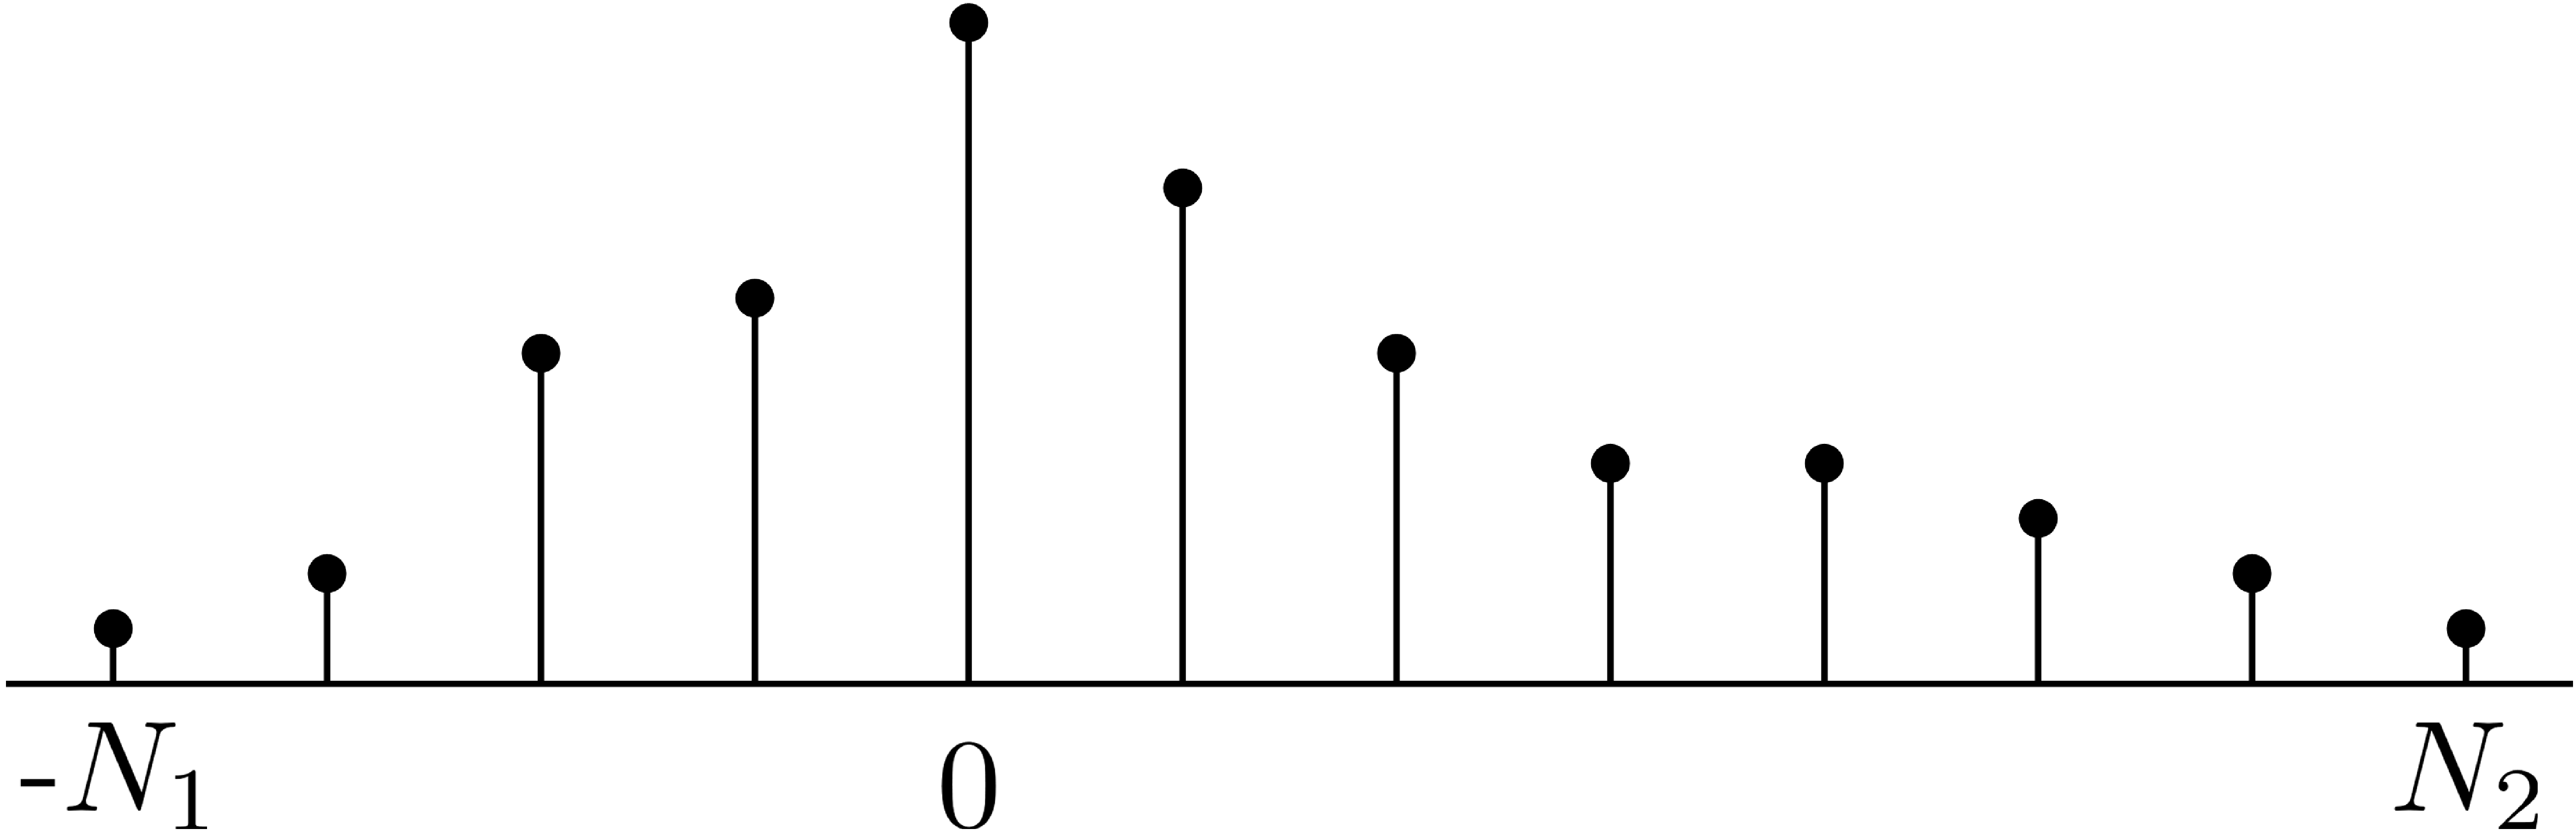
\includegraphics[width=5.5in/100*55]{figures/intro/channelExample.pdf}
	\caption{An illustration of the discrete-time channel of length $N_1+N_2+1$ with a non-causal component comprising $N_1$ samples and a causal component comprising $N_2$ samples.}
	\label{fig:channelExample}
\end{figure}

\subsubsection{Digital Signal Processing}
\label{sec:signalProcessing}
A high-level digital signal processing flow is shown in Figure \ref{fig:estimators} and \ref{fig:thisThesisBlock}.
Because the frequency offset, channel, and noise variance are estimated using the preamble and ASM, the first step is to find the samples correlating to the preamble in the received sample sequence $r(n)$.
The preamble detector block correlates received samples with $L_\text{P}$ samples of a locally stored copy of the pilot in \eqref{eq:preamble_ASM}.
The preamble detector block outputs the vector of samples $\mathbf{r}_\text{p}$ with the iNET packetized structure.
The first $L_\text{P} + L_\text{ASM}$ samples in $\mathbf{r}_\text{p}$ correlate with the received pilot samples.
\begin{equation}
\mathbf{p} = \big[ p(0) \quad p(1) \quad \cdots  \quad  p(L_\text{P} + L_\text{ASM}-1) \big]
\label{eq:preamble_ASM}
\end{equation}

The located preamble samples are used first to estimate the frequency offset.
The estimated frequency offset $\hat{\omega}_0$ rads/sample is then used to ``de-rotate'' the vector of samples $\mathbf{r}_\text{p}$ to produce $\mathbf{r}$.
The de-rotated samples in the vector $\mathbf{r}$ that correlate to the preamble and ASM are used to estimate the channel $\hat{\mathbf{h}}$ and noise variance $\hat{\sigma}^2_w$.
The channel and noise variance estimates are done in the estimators block.
\begin{figure}
	\centering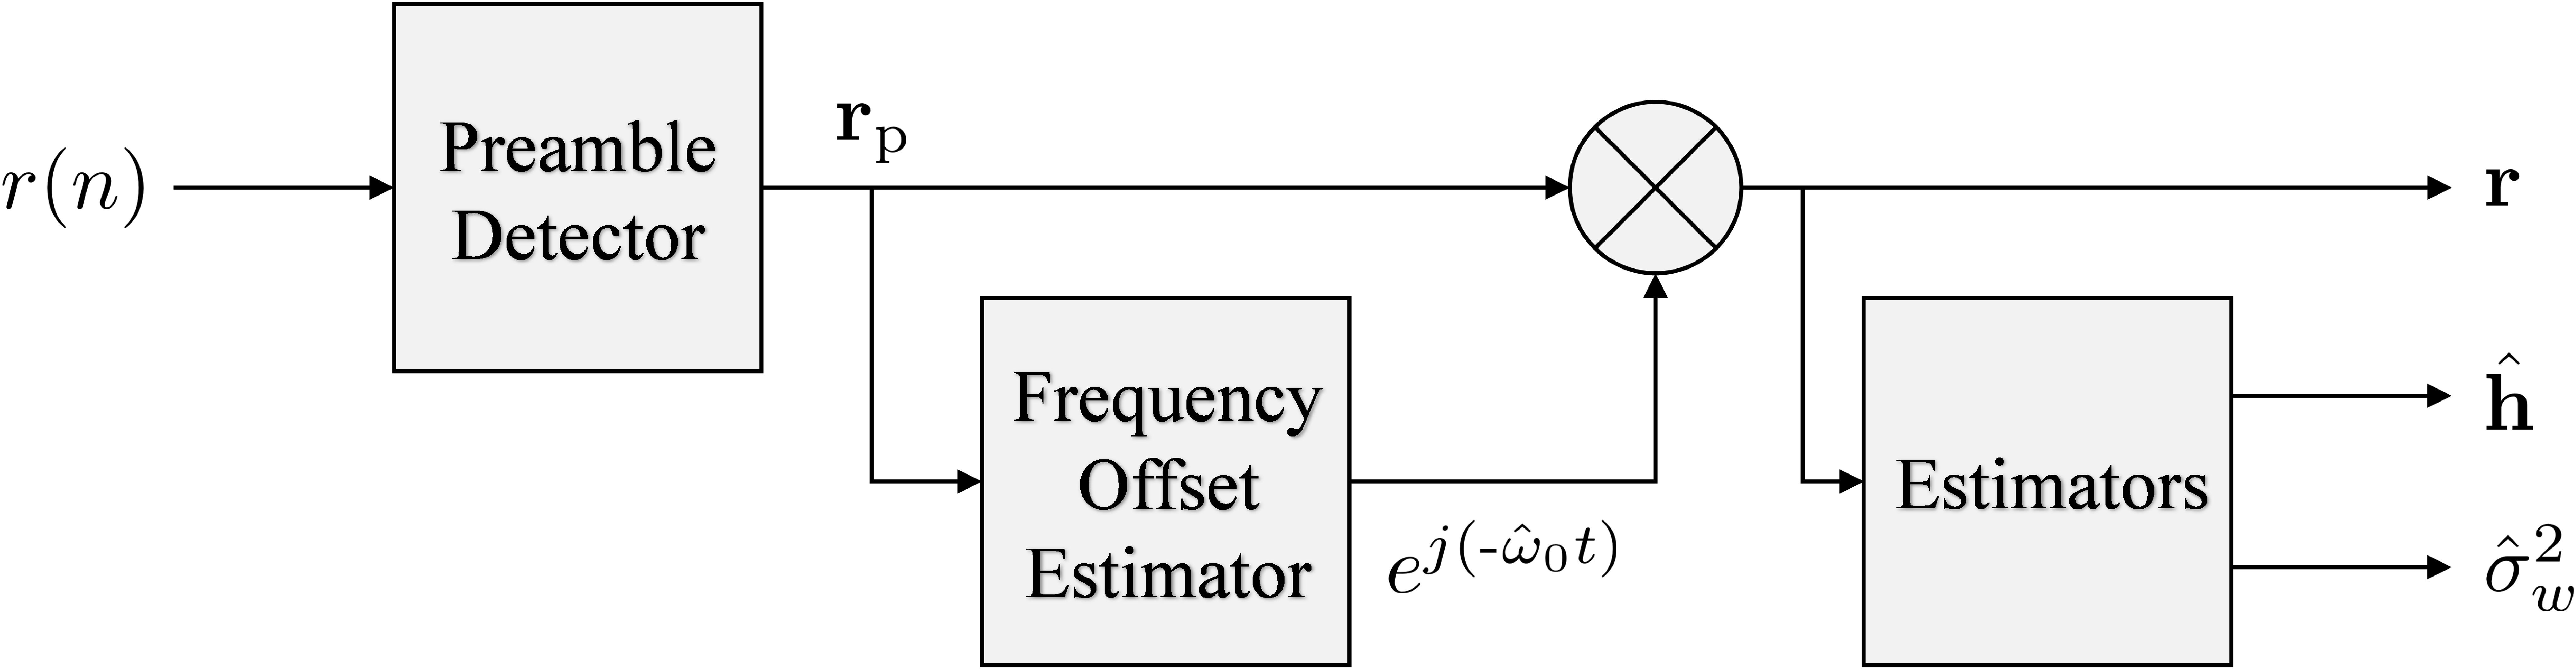
\includegraphics[width=8.75in/100*55]{figures/intro/estimators.pdf}
	\caption{A block diagram of the estimators in the PAQ project.}
	\label{fig:estimators}
\end{figure}

Equipped with knowledge of the estimated channel and noise variance, data-aided finite impulse response (FIR) equalizer filters can be computed.
The all the data-aided equalizer filters are computed using the same channel and noise variance estimates.
The blocks shown in Figure \ref{fig:thisThesisBlock} are duplicated in five independent branches producing five estimated vectors of bits $\hat{\mathbf{b}}$, one for each equalizer.

%An equalizer filter is computed using the channel estimate $\hat{\mathbf{h}}$ and noise variance $\hat{\sigma}^2_w$ then applied to the vector of samples $\mathbf{r}$.
The PAQ project designed the data-aided FIR equalizer filters to be $5$ times longer than the channel estimate. The equalizer filter has a non-causal component comprising $L_1 = 5N_1 = 60$ samples and a causal component comprising $L_2 = 5N_2 = 125$ samples.
The $L_\text{EQ} = L_1+L_2+1$ sample full discrete-time equalizer filters are computed and applied in the equalizer filter block.

The output of the equalizer filters are then filtered by a SOQPSK-TG detection filter and down-sampled by $2$ in preparation for an OQPSK detector.
The $\mathbf{r}_\text{d}$ in each equalizer branch has a sample rate of $1$ sample/bit or $2$ samples/symbol.
The OQPSK detector block outputs the vector of estimated bits $\hat{\mathbf{b}}$.
\begin{figure}
	\centering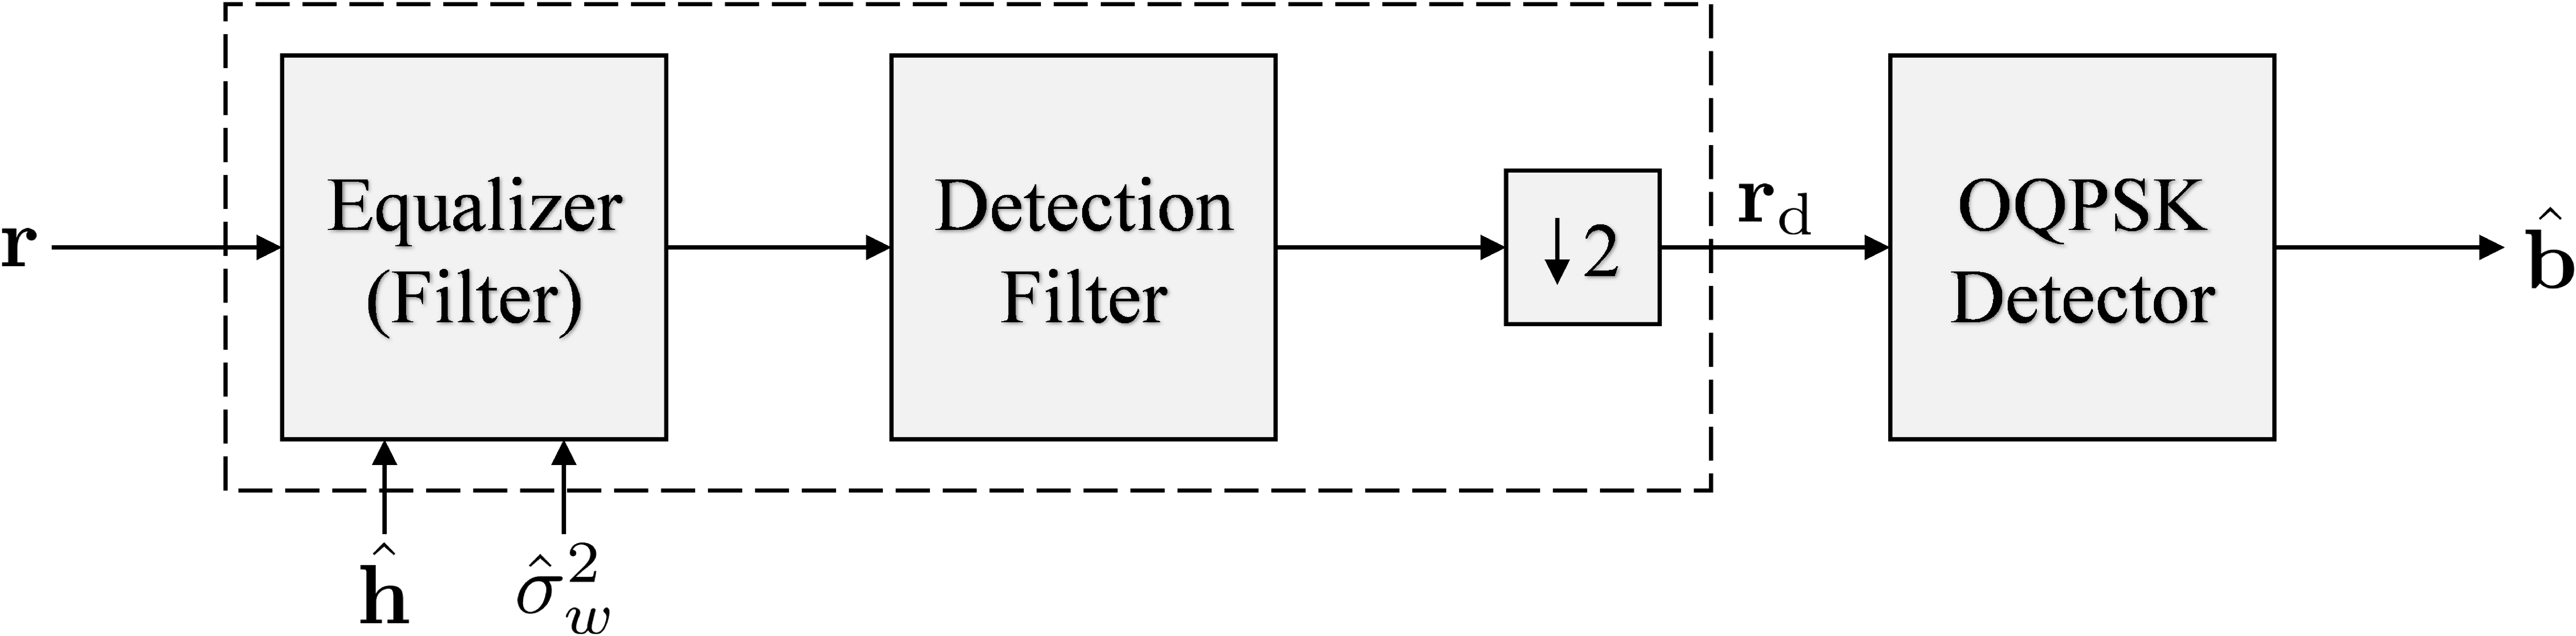
\includegraphics[width=8.37in/100*55]{figures/intro/thisThesisBlock.pdf}
	\caption{A block diagram of application of the FIR equalizer and detection filters in the Preamble Assisted Equalization (PAQ) project.}
	\label{fig:thisThesisBlock}
\end{figure}
Finally the BER for each equalizer is obtained by comparing the vectors of estimated bits $\hat{\mathbf{b}}$ to the PN sequence.

The GPUs in Figure \ref{fig:hardwareblock} and \ref{fig:HostSystem} perform all the digital signal processing in parallel.
To introduce as much parallelism as possible, the received samples are processed in $39$,$321$,$600$ sample 		sets. 
At $20.625$ Msamples/second, each set of $39$,$321$,$600$ samples is $1907$ milliseconds worth of data.
Each set has at most $3104$ independent $12672$ sample iNET packets.
The GPU processes $3104$ packets in parallel by leveraging batched processing.
Each packet is a batch and each batch performs the algorithms shown in Figures \ref{fig:estimators} and \ref{fig:thisThesisBlock}.
In order to stay real-time, \textbf{all} processing must be completed in $1907$ ms.

This thesis, will illustrate how the five PAQ data-aided equalizers were computed and applied to the received samples in GPUs.
The dashed box in Figure \ref{fig:thisThesisBlock} emphasizes which processing blocks are focused on.

Chapter \ref{chap:equations} shows the equations for these block diagrams.
Chapter \ref{chap:gpu} will shed some light on signal processing in GPUs.
Chapter \ref{chap:equalizers_in_gpus} will illustrate how the five equalizers are implemented in GPUs.
Chapter \ref{chap:final_summary} will summarize.